

\section{Evaluation}
\label{evaluation}

In this section, we evaluate the performance and power efficiency of Plasticine against a commercial Stratix V FPGA.
We compare the runtime and power of the Plasticine architecture to efficient FPGA implementations for benchmarks taken from the
machine learning, data analytics, and graph processing domains. %Compared to many proposed CGRAs, 
FPGAs are widely available with mature toolchain support, which makes it possible to obtain performance data on
real hardware.

% \todo{Do we want to keep this justification?}
% We justify evaluating against the FPGA as follows:
% \begin{itemize}
%   \item From the architectures in Table~\ref{t-related}, the only other spatial architecture supporting
%     a high-level programming interface that is flexible enough to allow mapping entire applications
%     with nested parallelism and custom on-chip data structures is the FPGA.
%   \item As discussed in Section~\ref{relatedWork}, reconfigurable architectures proposed in previous literature
%     differ widely in their granularities, target applications, architectural capabilities, compiler toolchains, and
%     programming models. Such heterogeneity is not suitable for direct quantitative comparisons that are fair and accurate.
% \end{itemize}

\subsection{Benchmarks}
\label{benchmarks}
%Points to mention:
% \begin{itemize}
%   \item FPGA setup:
%   \begin{itemize}
%     \item Maxeler, Altera specs
%     \item Performance: FPGA execution time including accesses to off-chip DRAM
%     \item Area: Altera place-and-route
%     \item Power: Altera PowerPlay
%   \end{itemize}
%   \item Plasticine setup:
%     \begin{itemize}
%       \item Architecture spec: \#PCUs, registers, BRAMs, memory channels, etc. Same off-chip memory interface as FPGA.
%       \item Logic synthesis spec: 45nm TSMC technology library, normalization to 28nm etc.
%     \end{itemize}
%     \begin{itemize}
%       \item Performance: Chisel simulation, DDR trace + DRAMSim2~\cite{dramsim2} for off-chip memory access.
%       \item Area: Post PAR from icc, CACTI, something for memory controller.
%       \item Power: Power compiler, CACTI, DRAMSim2
%     \end{itemize}
%   \item Benchmarks table. All benchmarks are written in SPATIAL. The same source is transformed to MaxJ for FPGA,
%     PISA for Plasticine.
% \end{itemize}

\begin{table}[]
\centering
\resizebox{0.955\columnwidth}{!}{
\begin{tabular}{@{}llll@{}}
\bottomrule
\textbf{Benchmark} & \textbf{Data Size(s)}                          & \textbf{Data Type} \\ \midrule
  Inner Product    & 768,000,000                                    & float32            \\ \midrule
  Outer Product    & 76,800 $\times$ 76,800                         & float32            \\ \midrule
  Black-Scholes    & 96,000,000 entries                             & float32            \\ \midrule
  TPC-H Query 6    & 960,000,000 entries                            & int32              \\ \midrule
  GEMM             & 47 $\times$ 7,680 * 7,680 $\times$ 3,840       & float32            \\ \midrule
  GDA              & 3,840,000 points; 96 dims                      & float32            \\ \midrule
  LogReg           & 5 iters; 1,536 points; 384 dims                & float32            \\ \midrule
  SGD              & 30 iters; 38,400 points; 768 dims              & float32            \\ \midrule
  Kmeans           & 50 iters; 1,536 points; 96 dims; K = 20        & float32            \\ \midrule
  CNN              & model size 884736, data size 57600             & float32            \\ \midrule
  SMDV             & 3,840 $\times$ 3,840 with $E[NNZ]_{node} = 60$ & float32            \\ \midrule
  PageRank         & 100 iters; 7,680 pages                         & int32              \\ \midrule
  BFS              & $E[edges]_{node} = 8$ $\times$ 10 layers       & int32              \\ \midrule
\end{tabular}
}
\caption{Evaluation benchmarks.}
\label{t-apps}
\vspace{-25pt}
\end{table}

  We developed a set of benchmarks that stress a variety of properties of the two architectures, such as dense data processing and data-dependent memory access.  We use real-world applications to guide the design of these benchmarks to ensure that Plasticine is capable of doing useful work.  
  Table~\ref{t-apps} provides a summary of the applications.  

  Among the dense applications, \textit{inner product}, \textit{outer product}, and \textit{GEMM} (single precision general matrix multiplication) are fundamental linear algebra operations
  and at the core of many algorithms.
  \textit{TPC-H Query 6} is a simple filter-reduce kernel that demonstrates database query functionality.
  \textit{Black-Scholes} is a computation-heavy finance algorithm with extremely deep pipelines.
  Gaussian Discriminant Analysis (\textit{GDA}) and Stochastic Gradient Descent (\textit{SGD}) are common machine learning algorithms that involve relatively complicated memory accesses and exhibit many choices for parallelization.
  \textit{K-means} clustering groups a set of input points by iteratively calculating the $k$ best cluster centroids.
  K-means is written using a dense HashReduce to calculate the next iteration's centroids.
  Convolutional Neural Network (\textit{CNN}) is an important machine learning kernel used for image classification. CNNs involve multiple layers of computation, where each layer involves several 3D convolution operations on an input feature map.

  The sparse applications involve data-dependent accesses to memory and non-deterministic computation.
  Sparse matrix-dense vector (\textit{SMDV}) multiplication is another fundamental linear algebra kernel used in many sparse iterative methods and optimization algorithms.
  \textit{PageRank} is a popular graph algorithm that involves off-chip sparse data gathering to iteratively update page rankings.
  Breadth-First Search (\textit{BFS}) is another graph algorithm that performs a data-dependent, frontier-based traversal and uses data scatters to store information about each node.




%\begin{table}[]
%\centering
%\begin{tabular}{l|cccc}
%\end{tabular}
%\caption{Plasticine architecture parameters}
%\end{table}

We implement each of these benchmarks in the Delite Hardware Definition Language (DHDL), 
a specialized language based on parallel patterns for writing applications for spatial architectures~\cite{dhdl}. In DHDL, applications are specified as hierarchies of parallelizable dataflow pipelines. Previous work~\cite{delite2maxj} has shown that DHDL can be automatically generated
from parallel patterns, and can be used to generate efficient hardware accelerator designs for FPGAs~\cite{dhdl}.



\subsection{Plasticine Design}


%\begin{table*}[]
%\centering
%\resizebox{0.8\textwidth}{!}{%
%\begin{tabular}{l|c|cr|cr|cr|cr}%|cr}
%\toprule
%\textbf{Benchmark} 
%& \textbf{\shortstack{\emph{a.} Coarse\\Units}}
%& \multicolumn{2}{c}{ \textbf{\shortstack{\emph{b.} Homogeneous\\PMUs}} }
%& \multicolumn{2}{|c}{ \textbf{\shortstack{\emph{c.} Homogeneous\\PCUs}} }
%& \multicolumn{2}{|c}{ \textbf{\shortstack{\emph{d.} Generalized\\PMUs}} }
%& \multicolumn{2}{|c}{ \textbf{\shortstack{\emph{e.} Generalized\\PCUs}} } \\ \midrule
%%& \multicolumn{2}{|c}{ \textbf{\shortstack{\emph{f.} Final\\Architecture}} } \\ \midrule

%Inner Product & \emph{2.64$\times$} & \emph{1.21$\times$} & (3.18$\times$) & \emph{2.66$\times$} &  (8.45$\times$) & \emph{1.53$\times$} & (12.92$\times$) & \emph{1.02$\times$} & (13.18$\times$) \\  %& \emph{3.24} & (42.66\times$) \\
%Outer Product & \emph{1.54$\times$} & \emph{2.07$\times$} & (3.18$\times$) & \emph{1.83$\times$} &  (5.81$\times$) & \emph{1.00$\times$} &  (5.81$\times$) & \emph{1.02$\times$} &  (5.95$\times$) \\  %& \emph{4.61} & (27.42$\times$) \\
%Black-Scholes & \emph{2.05$\times$} & \emph{1.05$\times$} & (2.15$\times$) & \emph{1.59$\times$} &  (3.43$\times$) & \emph{1.18$\times$} &  (4.04$\times$) & \emph{1.10$\times$} &  (4.46$\times$) \\  %& \emph{2.86} & (12.78$\times$) \\
%TPCH-Query 6  & \emph{2.26$\times$} & \emph{1.15$\times$} & (2.59$\times$) & \emph{3.90$\times$} & (10.10$\times$) & \emph{1.24$\times$} & (12.49$\times$) & \emph{1.15$\times$} & (14.32$\times$) \\  %& \emph{2.82} & (40.44$\times$) \\
%GEMM          & \emph{1.63$\times$} & \emph{1.45$\times$} & (2.36$\times$) & \emph{1.62$\times$} &  (3.82$\times$) & \emph{1.00$\times$} &  (3.83$\times$) & \emph{1.02$\times$} &  (3.92$\times$) \\  %& \emph{2.95} & (11.56$\times$) \\
%GDA           & \emph{1.95$\times$} & \emph{1.79$\times$} & (3.50$\times$) & \emph{3.03$\times$} & (10.59$\times$) & \emph{1.34$\times$} & (14.19$\times$) & \emph{1.01$\times$} & (14.38$\times$) \\  %& \emph{1.43} & (20.60$\times$) \\
%LogReg        & \emph{1.55$\times$} & \emph{1.91$\times$} & (2.96$\times$) & \emph{1.73$\times$} &  (5.12$\times$) & \emph{1.00$\times$} &  (5.13$\times$) & \emph{1.02$\times$} &  (5.20$\times$) \\  %& \emph{1.80} & (9.36$\times$) \\
%SGD           & \emph{7.67$\times$} & \emph{1.09$\times$} & (8.40$\times$) & \emph{1.82$\times$} & (15.31$\times$) & \emph{1.41$\times$} & (21.61$\times$) & \emph{1.02$\times$} & (21.98$\times$) \\  %& \emph{17.12} & (376.23$\times$) \\
%Kmeans        & \emph{2.81$\times$} & \emph{1.88$\times$} & (5.29$\times$) & \emph{1.74$\times$} &  (9.19$\times$) & \emph{1.00$\times$} &  (9.20$\times$) & \emph{1.02$\times$} &  (9.42$\times$) \\  %& \emph{9.56} & (90.02$\times$) \\
%SMDV          & \emph{5.03$\times$} & \emph{1.24$\times$} & (6.26$\times$) & \emph{4.04$\times$} & (25.31$\times$) & \emph{1.36$\times$} & (34.51$\times$) & \emph{1.06$\times$} & (36.73$\times$) \\  %& \emph{1.86} & (68.30$\times$) \\
%PageRank      & \emph{7.14$\times$} & \emph{1.18$\times$} & (8.41$\times$) & \emph{3.39$\times$} & (28.51$\times$) & \emph{1.46$\times$} & (41.73$\times$) & \emph{1.03$\times$} & (42.83$\times$) \\  %& \emph{3.00} & (128.54$\times$) \\
%BFS           & \emph{2.91$\times$} & \emph{1.38$\times$} & (4.02$\times$) & \emph{2.14$\times$} &  (8.61$\times$) & \emph{1.21$\times$} & (10.40$\times$) & \emph{1.03$\times$} & (10.70$\times$) \\ \midrule  %& \emph{5.08} & (54.38$\times$) \\ \midrule
%GeoMean       & \emph{2.77$\times$} & \emph{1.41$\times$} & (3.92$\times$) & \emph{2.32$\times$} &  (9.07$\times$) & \emph{1.21$\times$} & (11.00$\times$) & \emph{1.04$\times$} & (11.46$\times$) \\ \bottomrule %& \emph{7.64} & (87.56$\times$) \\ \bottomrule
%\end{tabular}
%}
%\caption{Estimated \emph{successive} and (cumulative) area overheads of \emph{a.}~generalizing ASICs into reconfigurable, heterogeneous PCUs and PMUs; \emph{b.}~restricting the architecture to homogeneous PMUs; \emph{c.} further restricting the architecture to homogeneous PCUs; \emph{d.}~generalizing homogeneous PMUs across applications; \emph{e.}~generalizing homogeneous PCUs across applications.
%} %; \emph{f.}~fixing the size of the architecture to the final 16$\times$8 units.}
%\label{t-area_overheads}
%\vspace{-10pt}
%\end{table*}

We implement the Plasticine architecture in Chisel~\cite{chisel} using the selected parameters listed in Table~\ref{t-parameters}.
The architecture is organized as a 16$\times$8 array of units, with a 1:1 ratio of PMUs to PCUs.
This design is synthesized using Synopsys Design Compiler with a 28nm technology library.
Critical paths in the design have been optimized for a clock frequency of 1 GHz.
Total chip area estimates are obtained after synthesis. Local scratchpad and FIFO sizes are obtained using
Synopsys Memory Compiler with a 28nm library. We profile single PCU, PMU, and AG power using Synopsys
PrimeTime with RTL traces. Static power for the entire chip and dynamic power for utilized units are
included in the total power.
%We report chip area and power normalized to 28~nm for direct comparison to the Stratix V FPGA.
Table~\ref{t-breakdown} provides the component-wise area breakdown for Plasticine at an area footprint of 112.77$mm^2$. The final Plasticine architecture has a peak floating point performance of 12.3 single-precision ~TFLOPS and a total on-chip scratchpad capacity of 16~MB.

Execution times for Plasticine are obtained from cycle-accurate simulations performed using Synopsys VCS coupled with DRAMSim2~\cite{dramsim2}
to measure off-chip memory access times. We configure DRAMSim2 to model a memory system with 4 DDR3-1600 channels, giving a theoretical peak
bandwidth of 51.2 GB/s.

We modify the DHDL compiler to generate static configurations for Plasticine using the procedure outlined in Section~\ref{mapping}.
Using the modified compiler, each benchmark is compiled to a Plasticine configuration, which is used to program the simulator.
Total reported runtime for Plasticine begins after data is copied into the accelerator's main memory,
and ends when execution on the accelerator is complete (i.e. before copying data back to the host).

%\subsection{Area and Power}

\begin{table}[]
\centering
\resizebox{\columnwidth}{!}{%


\begin{tabular}{ll S[table-format=3.3] S[table-format=3.2]}
\toprule
                                                                              & Component              & {Area $(mm^2)$} & {Area $(\%)$} \\ \midrule
\multirow{5}{*}{\shortstack[l]{PCU\\(48.16\%)}}                               & FUs                    & 0.622    & 73.32  \\
                                                                              & Registers              & 0.144    & 16.97  \\
                                                                              & FIFOs                  & 0.082    & 9.65   \\
                                                                              & Control                & 0.001    & 0.06   \\
                                                                              & \emph{Total (single PCU)}     & 0.849    & 100.00 \\ \midrule
\multirow{5}{*}{\shortstack[l]{PMU\\(30.2\%)}}                                & Scratchpad (256KB)     & 0.477    & 89.73  \\
                                                                              & FIFOs                  & 0.024    & 4.52   \\
                                                                              & Registers              & 0.023    & 4.28   \\
                                                                              & FUs                    & 0.007    & 1.29   \\
                                                                              & Control                & 0.001    & 0.18   \\
                                                                              & \emph{Total (single PMU)}     & 0.532    & 100.00 \\ \midrule
\multirow{2}{*}{\shortstack[l]{Interconnect\\(16.66\%)}}                      &                                          \\
                                                                              &                        & 18.796   & 100.00     \\ \midrule
\multirow{2}{*}{\shortstack[l]{Memory Controller\\(4.98\%)}}                  & 4 Coalescing Units,    &          &             \\
                                                                              & 34 AGs                 & 5.616    & 100.00      \\ \midrule
Plasticine                                                                    & 64 PCUs, 64 PMUs, &          &      \\
                                                                              & Memory Controller,     &           & \\
                                                                              & Interconnect & 112.796  & 100.00     \\ \bottomrule
\end{tabular}
}

\caption{Plasticine area breakdown.}
\label{t-breakdown}
\vspace{-25pt}
\end{table}


%Functional units, registers, and scratchpad memories comprise most of the area
%in a PCU. % Control logic accounts for less than 3 of the overall PCU area.





\subsection{Plasticine Design Overheads}
We first examine the area overheads of design decisions within the Plasticine architecture.
Each decision is isolated and evaluated based on an idealized architecture. 
These architectures are normalized such that, given a 1 GHz clock and fixed local memory sizes, 
the performance of each benchmark is the same as its performance on the final Plasticine architecture.
These design decisions (columns~\emph{a.}~---~\emph{e.} in Table~\ref{t-area_overheads}) allow an arbitrary number of PCUs and PMUs for each benchmark.
This is done to isolate the quality of the choice from an application's utilization of a fixed size architecture.  

We first evaluate the cost of partitioning an application into coarse-grain PCUs and PMUs. 
Here, we compare the projected areas of benchmark-specific ASIC designs to an idealistic Plasticine architecture with \emph{heterogeneous} PCUs and PMUs.
For a given benchmark, ASIC area is estimated as the sum of the area of its compute and memory resources. The area of each of these resources was characterized using Synopsys DC.
The Plasticine architecture has all of the features described in Section~\ref{plasticine}, including configuration logic, configurable banked memories, and statically configurable ALUs.
Column~\emph{a.} of Table~\ref{t-area_overheads} shows the projected costs of such a heterogeneous architecture relative to the projected area of the benchmark-specific chip design. 
Relative to ASIC designs, the area overhead of reconfigurable units is on average about 2.8$\times$. This is the base overhead of Plasticine's reconfigurability, 
primarily concentrated in making memory controllers configurable and converting compute logic from fixed operations to reconfigurable~FUs.


\begin{table}[]
\centering
\resizebox{1\columnwidth}{!}{%
\begin{tabular}{l|c|cr|cr|cr|cr}%|cr}
\toprule
& \textbf{Coarse} & \multicolumn{4}{c|}{ \textbf{\shortstack{Homogeneous}} } & \multicolumn{4}{c}{ \textbf{\shortstack{Generalized}} } \\
\textbf{Benchmark} 
& \textbf{\emph{a.}}
& \multicolumn{2}{c}{ \textbf{\shortstack{\emph{b.} PMUs}} }
& \multicolumn{2}{c|}{ \textbf{\shortstack{\emph{c.} PCUs}} }
& \multicolumn{2}{c}{ \textbf{\shortstack{\emph{d.} PMUs}} }
& \multicolumn{2}{c}{ \textbf{\shortstack{\emph{e.} PCUs}} } \\ \midrule
%& \multicolumn{2}{|c}{ \textbf{\shortstack{\emph{f.} Final\\Architecture}} } \\ \midrule

Inner Product & \emph{2.64} & \emph{1.21} & (3.18) & \emph{2.66} &  (8.45) & \emph{1.53} & (12.92) & \emph{1.02} & (13.18) \\  %& \emph{3.24} & (42.66\times$) \\
Outer Product & \emph{1.54} & \emph{2.07} & (3.18) & \emph{1.83} &  (5.81) & \emph{1.00} &  (5.81) & \emph{1.02} &  (5.95) \\  %& \emph{4.61} & (27.42) \\
Black-Scholes & \emph{2.05} & \emph{1.05} & (2.15) & \emph{1.59} &  (3.43) & \emph{1.18} &  (4.04) & \emph{1.10} &  (4.46) \\  %& \emph{2.86} & (12.78) \\
TPCH-Query 6  & \emph{2.26} & \emph{1.15} & (2.59) & \emph{3.90} & (10.10) & \emph{1.24} & (12.49) & \emph{1.15} & (14.32) \\  %& \emph{2.82} & (40.44) \\
GEMM          & \emph{1.63} & \emph{1.45} & (2.36) & \emph{1.62} &  (3.82) & \emph{1.00} &  (3.83) & \emph{1.02} &  (3.92) \\  %& \emph{2.95} & (11.56) \\
GDA           & \emph{1.95} & \emph{1.79} & (3.50) & \emph{3.03} & (10.59) & \emph{1.34} & (14.19) & \emph{1.01} & (14.38) \\  %& \emph{1.43} & (20.60) \\
LogReg        & \emph{1.55} & \emph{1.91} & (2.96) & \emph{1.73} &  (5.12) & \emph{1.00} &  (5.13) & \emph{1.02} &  (5.20) \\  %& \emph{1.80} & (9.36) \\
SGD           & \emph{7.67} & \emph{1.09} & (8.40) & \emph{1.82} & (15.31) & \emph{1.41} & (21.61) & \emph{1.02} & (21.98) \\  %& \emph{17.12} & (376.23) \\
Kmeans        & \emph{2.81} & \emph{1.88} & (5.29) & \emph{1.74} &  (9.19) & \emph{1.00} &  (9.20) & \emph{1.02} &  (9.42) \\  %& \emph{9.56} & (90.02) \\
SMDV          & \emph{5.03} & \emph{1.24} & (6.26) & \emph{4.04} & (25.31) & \emph{1.36} & (34.51) & \emph{1.06} & (36.73) \\  %& \emph{1.86} & (68.30) \\
PageRank      & \emph{7.14} & \emph{1.18} & (8.41) & \emph{3.39} & (28.51) & \emph{1.46} & (41.73) & \emph{1.03} & (42.83) \\  %& \emph{3.00} & (128.54) \\
BFS           & \emph{2.91} & \emph{1.38} & (4.02) & \emph{2.14} &  (8.61) & \emph{1.21} & (10.40) & \emph{1.03} & (10.70) \\ \midrule  %& \emph{5.08} & (54.38) \\ \midrule
GeoMean       & \emph{2.77} & \emph{1.41} & (3.92) & \emph{2.32} &  (9.07) & \emph{1.21} & (11.00) & \emph{1.04} & (11.46) \\ \bottomrule %& \emph{7.64} & (87.56) \\ \bottomrule
\end{tabular}
}
\caption{Estimated \emph{successive} and (cumulative) area overheads of \emph{a.}~generalizing ASICs into reconfigurable, heterogeneous PCUs and PMUs; \emph{b.}~restricting the architecture to homogeneous PMUs; \emph{c.} further restricting the architecture to homogeneous PCUs; \emph{d.}~generalizing homogeneous PMUs across applications; \emph{e.}~generalizing homogeneous PCUs across applications.
} %; \emph{f.}~fixing the size of the architecture to the final 16$\times$8 units.}
\label{t-area_overheads}
\vspace{-20pt}
\end{table}


While use of heterogeneous units is ideal for area utilization, it creates an intractable mapping problem and does not generalize across different applications. 
In column~\emph{b.} of Table~\ref{t-area_overheads}, we show the cost of moving from a heterogeneous architecture to an architecture still with heterogeneous PCUs 
but a single homogeneous PMU design. We still allow this PMU design to be unique for each benchmark, but within a single benchmark we size
the PMU scratchpads based on the largest scratchpad the program requires.
The average overhead from moving to uniform PMUs is 1.4$\times$, with particularly large overheads for applications with drastically varying memory sizes.
OuterProduct, for example, uses local memories for tiles of vectors of size $N$ and an output tile of size $N^2$.
In ASIC design, static knowledge about the target application allows specialization of each local memory to exactly the size and number of banks needed, 
thus saving a significant amount of area on SRAM. 
In Plasticine, we opt for uniformly sized memory units as they simplify mapping and improve the likelihood that a given application will be routable.

Column~\emph{c.} shows the overheads of further restricting the PCUs to also be homogeneous, but still vary across benchmarks.
The overhead here is particularly high for applications like PageRank with a large number of sequential loops. 
The bodies of all patterns are mapped to PCUs, but because each PCU is fixed to 16 lanes, most of the lanes in sequential loops, and therefore most of the area, is unused, 
leading to overheads of up to 8.4$\times$.
Similarly, applications like TPCHQ6 with widely varying compute pipeline lengths tend to under-utilize the stages within homogeneous PCUs.

We next show the area overheads after selecting a single set of PMU parameters across all applications. 
As described in Section~\ref{sizing_section}, this sets the total size of scratchpads in all benchmarks to 256KB each.
While this local memory capacity is essential to the performance of applications like GEMM and OuterProduct \cite{LAP_TC12}, other applications have much smaller local memory requirements.
As seen in column~\emph{d}, this unutilized SRAM capacity has an average chip area overhead of 1.2$\times$.

Column~\emph{e.} lists the results of also generalizing PCUs across applications using the values obtained in Section~\ref{sizing_section}.
Here, we see that the remaining overhead is small compared to the cost of homogenizing the units, with an average of only 5\% and a maximum of 15\% for BlackScholes.
This suggests that much of the variation in PCU requirements across applications is already represented by the variety of loops within a single application.
This in turn makes generalization of compute across applications relatively inexpensive.

Cumulatively, we estimate that our homogeneous, generalized, unit based architecture has an average area overhead of 3.9$\times$ to 42.8$\times$ compared to application-specific chip designs with the same performance. 
This overhead of course varies significantly based on the local memory and compute requirements of the benchmark.
While the PCU and PMU utilizations of the final, fixed size Plasticine architecture, later shown in Table~\ref{t-comparision}, tend to be less than 100\%, we do not view this in itself as an area overhead. 
Instead, the Plasticine architecture is considered a ``sufficiently large'' fabric which can be used to 
implement the ideal architectures listed in column~\emph{e.}, and the remaining unit resources can be clock gated.

%Finally, column \emph{f.} gives the area overheads due to fixing the number of PCUs and PMUs in the architecture.
%This additional overhead is directly related to each benchmarks total utilization given in Table~\ref{t-utilization}. 
%Cumulatively, we estimate that the final Plasticine architecture has an average area overhead of \todo{?? $\times$} to \todo{?? $\times$} compared to application-specific chip designs with the same performance. This overhead of course varies significantly based on the local memory and compute requirements of the benchmark.

\subsection{FPGA Design}

We next compare the performance and power of Plasticine to an FPGA.
We use the DHDL compiler to generate VHDL, which in turn is used to generate a bitstream for the FPGA using Altera's synthesis tools.
We run each synthesized benchmark on an Altera~28nm Stratix~V FPGA, which interfaces with a host CPU controller via PCIe.
The FPGA has a 150 MHz fabric clock, a 400 MHz memory controller clock, and 48 GB of dedicated off-chip DDR3-800 DRAM with 6 channels and a peak bandwidth of 37.5 GB/s.
Execution times for the FPGA are reported as an average of 20 runs. Like Plasticine, timing starts after copy of data from the host to the FPGA's dedicated DRAM completes and finishes when FPGA execution completes. We also obtain FPGA power estimates for each benchmark using Altera's PowerPlay tool after benchmark placement and routing.

\subsection{Plasticine versus FPGA}

%\begin{table}[]
%\centering
%\resizebox{\columnwidth}{!}{%
%\begin{tabular}{l|ccccc}
%\toprule
%\textbf{Benchmark} & \textbf{Speedup} & \textbf{\shortstack{FPGA \\ Power (W)}} & \textbf{\shortstack{Plasticine \\ Power (W)}} & \textbf{\shortstack{Normalized\\ Power}} & \textbf{\shortstack{Normalized \\ Perf/W}} \\ \midrule
	%Inner Product    & 1.36             &  21.82                  &  18.96                        & 0.87                                     & 1.56  \\
	%Outer Product    & 6.71             &  24.35                  &  26.88                        & 1.10                                     & 6.08  \\
	%Black-Scholes    & 5.05             &  28.29                  &  24.74                        & 0.87                                     & 5.77  \\
	%TPCH-Query 6     & 1.39             &  21.74                  &  20.53                        & 0.94                                     & 1.48  \\
	%GEMM             & 32.96            &  25.62                  &  34.61                        & 1.35                                     & 24.40 \\
	%GDA              & 39.99            &  26.54                  &  41.00                        & 1.54                                     & 25.90 \\
	%LogReg           & 11.44            &  22.96                  &  28.64                        & 1.25                                     & 9.17  \\
	%SGD              & 6.67             &  25.58                  &  10.73                        & 0.42                                     & 15.89 \\
	%Kmeans           & 6.08             &  23.90                  &  12.91                        & 0.54                                     & 11.26 \\
	%CNN              & 95.14            &  34.45                  &  42.62                        & 1.24                                     & 76.91 \\
	%SMDV             & 8.31             &  21.48                  &  19.28                        & 0.90                                     & 9.26  \\
	%PageRank         & 14.19            &  21.99                  &  17.10                        & 0.78                                     & 18.25 \\
	%BFS              & 7.28             &  21.93                  &  14.01                        & 0.64                                     & 11.39 \\
%\bottomrule
%\end{tabular}
%}

%\caption{Comparison between FPGA and Plasticine based on performance, power, and performance per Watt.}
%\label{t-perf_summary}
%\vspace{-20pt}
%\end{table}

%\begin{table}[]
%\centering
%\resizebox{\columnwidth}{!}{%
%\begin{tabular}{l|cc|ccccc}
%\toprule
                     %&  \multicolumn{2}{c|}{\textbf{FPGA (\%)}}   &     \multicolumn{5}{c}{\textbf{Plasticine (\%)}}  \\ %\midrule
%\textbf{Benchmark} & \textbf{Logic} & \textbf{Memory} & \textbf{PCU} & \textbf{PMU} & \textbf{AG} & \textbf{FU} & \textbf{Register} \\ \midrule %       & \textbf{Ins} (\%) & \textbf{Outs} (\%)
%Inner Product      & 24.34          & 33.46           & 17.19        & 25.00        & 47.06          & 69.81       & 10.15                \\ %             & 41.75             & 24.50 \\
%Outer Product      & 38.19          & 71.37           & 15.63        & 46.88        & 88.24          & 21.62       & 12.84                \\ %             & 46.00             & 24.50 \\
%Black-Scholes      & 68.91          & 100.0           & 65.63        & 21.88        & 41.18          & 25.07       & 53.41                \\ %             & 60.75             & 50.00 \\
%TPCH-Query 6       & 24.29          & 33.35           & 28.13        & 25.00        & 47.06          & 70.80       & 20.17                \\ %             & 41.25             & 27.92 \\
%GEMM               & 40.44          & 94.78           & 34.38        & 68.75        & 97.06          & 56.02       & 8.60                 \\ %             & 41.50             & 30.00 \\
%GDA                & 53.61          & 96.84           & 89.06        & 87.50        & 44.12          & 8.13        & 11.16                \\ %             & 44.50             & 30.50 \\
%LogReg             & 28.42          & 73.35           & 51.56        & 68.75        & 8.82           & 30.24       & 12.26                \\ %             & 45.00             & 25.00 \\
%SGD                & 60.08          & 58.20           & 6.25         & 9.38         & 8.82           & 34.26       & 7.17                 \\ %             & 45.50             & 28.50 \\
%Kmeans             & 42.07          & 65.41           & 10.94        & 17.19        & 8.82           & 35.48       & 10.86                \\ %             & 41.75             & 33.15 \\
%CNN                & 86.82          & 99.00           & 48.96        & 98.4         & 100.00         & 62.50       & 25.00                \\ %             & 20.45             & 20.45 \\
%SMDV               & 27.33          & 31.01           & 43.75        & 15.63        & 29.41          & 10.38       & 2.67                 \\ %             & 37.00             & 29.25 \\
%PageRank           & 31.32          & 33.42           & 28.13        & 20.31        & 20.59          & 3.89        & 1.86                 \\ %             & 51.38             & 27.50 \\
%BFS                & 25.27          & 45.85           & 18.75        & 15.63        & 11.76          & 3.10        & 1.48                 \\ \bottomrule % & 41.67             & 23.33 \\ \bottomrule
%\end{tabular}
%}

%\caption{Plasticine and FPGA resource utilization breakdown by benchmark.}
%\label{t-utilization}
%\vspace{-20pt}
%\end{table}

\begin{table*}[]
\centering
\resizebox{0.9\textwidth}{!}{%
\begin{tabular} {l|S[table-format=2.1] S[table-format=3.1] | S[table-format=2.1] S[table-format=2.1] S[table-format=3.1] S[table-format=2.1] S[table-format=2.1]| S[table-format=2.1] S[table-format=2.1] | S[table-format=2.1] S[table-format=1.1] S[table-format=2.1] }
\toprule
& \multicolumn{7}{c|}{\textbf{Utilization (\%)}} 
& \multicolumn{2}{c|}{\textbf{Power (W)}} 
& \multicolumn{3}{c}{\textbf{Plasticine / FPGA}} \\


& \multicolumn{2}{c}{\textbf{FPGA}}
& \multicolumn{5}{c|}{\textbf{Plasticine}} 
& \multicolumn{1}{c}{\textbf{FPGA}} 
& \multicolumn{1}{c|}{\textbf{Plasticine}}
& \multicolumn{3}{c}{\textbf{ }} \\ %\midrule

{\textbf{Benchmark} } & 
{\textbf{Logic} } & 
{\textbf{Memory} } & 
{\textbf{PCU} } & 
{\textbf{PMU} } & 
{\textbf{AG} } & 
{\textbf{FU} } & 
{\textbf{Register} } & 
{} & 
{} &
{\textbf{Power}   } & 
{\textbf{Performance} } & 
{\textbf{Perf/W}  } \\ \midrule %       & \textbf{Ins} (\%) & \textbf{Outs} (\%)

Inner Product      & 24.3          & 33.5           & 17.2        & 25.0        & 47.1          & 69.8       & 10.2   & 21.8  & 18.9 & 0.9 & 1.4  & 1.6         \\ %             & 41.75             & 24.50 \\
Outer Product      & 38.2          & 71.4           & 15.6        & 46.9        & 88.2          & 21.6       & 12.8   & 24.4  & 26.9 & 1.1 & 6.7  & 6.1         \\ %             & 46.00             & 24.50 \\
Black-Scholes      & 68.9          & 100.0          & 65.6        & 21.9        & 41.2          & 25.1       & 53.4   & 28.3  & 24.7 & 0.9 & 5.1  & 5.8         \\ %             & 60.75             & 50.00 \\
TPCH-Query 6       & 24.3          & 33.4           & 28.1        & 25.0        & 47.1          & 70.8       & 20.2   & 21.7  & 20.5 & 0.9 & 1.4  & 1.5         \\ %             & 41.25             & 27.92 \\
GEMM               & 40.4          & 94.8           & 34.4        & 68.8        & 97.1          & 56.0       & 8.6    & 25.6  & 34.6 & 1.4 & 33.0 & 24.4        \\ %             & 41.50             & 30.00 \\
GDA                & 53.6          & 96.8           & 89.1        & 87.5        & 44.1          & 8.1        & 11.2   & 26.5  & 41.0 & 1.5 & 40.0 & 25.9        \\ %             & 44.50             & 30.50 \\
LogReg             & 28.4          & 73.4           & 51.6        & 68.8        & 8.8           & 30.2       & 12.3   & 22.9  & 28.6 & 1.2 & 11.4 & 9.2         \\ %             & 45.00             & 25.00 \\
SGD                & 60.1          & 58.2           & 6.3         & 9.4         & 8.8           & 34.3       & 7.2    & 25.6  & 10.7 & 0.4 & 6.7  & 15.9        \\ %             & 45.50             & 28.50 \\
Kmeans             & 42.1          & 65.4           & 10.9        & 17.2        & 8.8           & 35.5       & 10.9   & 23.9  & 12.9 & 0.5 & 6.1  & 11.3        \\ %             & 41.75             & 33.15 \\
CNN                & 86.8          & 99.0           & 48.9        & 98.4        & 100.0         & 62.5       & 25.0   & 34.4  & 42.6 & 1.2 & 95.1 & 76.9        \\ %             & 20.45             & 20.45 \\
SMDV               & 27.3          & 31.0           & 43.8        & 15.6        & 29.4          & 10.4       & 2.7    & 21.5  & 19.3 & 0.9 & 8.3  & 9.3         \\ %             & 37.00             & 29.25 \\
PageRank           & 31.3          & 33.4           & 28.1        & 20.3        & 20.6          & 3.9        & 1.9    & 21.9  & 17.1 & 0.8 & 14.2 & 18.2        \\ %             & 51.38             & 27.50 \\
BFS                & 25.3          & 45.9           & 18.8        & 15.6        & 11.8          & 3.1        & 1.5    & 21.9  & 14.0 & 0.6 & 7.3  & 11.4        \\ \bottomrule % & 41.67             & 23.33 \\ \bottomrule
\end{tabular}
}

	\caption{Resource utilization, power, performance, and performance-per-Watt comparisons between Plasticine and FPGA.}
\label{t-comparision}
\vspace{-20pt}
\end{table*}

Table~\ref{t-comparision} shows the utilization, power, performance, and performance-per-Watt of Plasticine relative to the Stratix V FPGA across our set of benchmarks.
The table shows that Plasticine achieves higher energy efficiency over an FPGA.
Table~\ref{t-comparision} shows the resource utilization on both platforms for each benchmark.
We discuss individual benchmark results below.
%In general, the power consumption of Plasticine is \todo{3$\times$ to 4$\times$} higher than the FPGA. \todo{However, with the exception of TPC-H Query 6, we see that our total energy consumption for each benchmark, equivalent to the performance per Watt, is better than the FPGA. 
%This is because the improved performance of Plasticine generally exceeds its higher power consumption.}

Inner product and TPC-H Query 6 both achieve speedups of 1.4$\times$, respectively. Both benchmarks are memory bandwidth bound,
where a large amount of data is streamed from DRAM through a datapath with minimal compute.
Hence, the performance difference corresponds to the difference in the achievable main memory bandwidth on the respective platforms.
The power consumption on Plasticine is comparable to the FPGA as well, as a majority of PCUs and half the PMUs are unused and therefore power gated.

Outer product is also bandwidth bound, but contains some temporal locality, and hence can benefit from larger tile sizes. The FPGA is limited by the number of large memories with
many ports that it can instantiate, which in turn limits exploitable inner loop parallelism and potential overlap between compute and DRAM communication.
Native support for banked, buffered scratchpads allows Plasticine to better exploit SIMD and pipelined parallelism, thereby achieving a speedup of 6.7$\times$.
%We see on Plasticine we have a speedup on these benchmarks of \todo{5.5$\times$, 3.7$\times$, and 1.9$\times$}, respectively.
%\todo{While the benchmarks are memory bound, the specialized memory controllers and local scratchpads allow us to make better use of the DRAM bandwidth as compared to the
%``soft'' memory controllers instantiated on the FPGA. 
%However, these benchmarks are still limited to an improvement in energy consumption of less than 1.5$\times$.}

Black-Scholes streams several floating point arrays from DRAM through a pipeline of floating point operations. The large amount of floating point
operations per DRAM access makes it compute-bound on most architectures. While the deeply pipelined nature of Black-Scholes makes it an ideal candidate for FPGA
acceleration, the FPGA runs out of area to instantiate compute resources long before it can saturate its main memory bandwidth. Plasticine, on the other hand,
has a much higher floating point unit capacity. Black-Scholes on Plasticine can be sufficiently parallelized to the point of being memory bound. From Table~\ref{t-comparision},
we can see that using 65\% of PCUs, Black-Scholes maximizes DRAM bandwidth utilization, achieving a
speedup of 5.1$\times$. 

GEMM and GDA are compute-bound, with ample temporal and spatial locality. On Plasticine, GEMM achieves a speedup of 33.0$\times$. GDA performs similarly
with a speedup of 40.0$\times$.
Plasticine can exploit greater locality by loading larger tiles into the banked scratchpads, and hides DRAM communication latency
by configuring scratchpads as double buffers. On the FPGA, creating banked, double-buffered tiles exhausts BRAM resources before compute resources, thereby
limiting compute throughput.
In the current mapping of GEMM to Plasticine, each PCU multiplies two tiles by successively performing pipelined inner products in its datapath. Parallelism is achieved within the PCU across the lanes,
and across PCUs where multiple tiles are processed in parallel. More parallelism is achieved by processing more input tiles in parallel. As a result, in the current scheme
GEMM performance is limited by the number of AGs, as more AGs are required to load multiple input tiles.
In addition, since each PCU performs an inner product, FUs that are not part of the reduction network are under-utilized.
More sophisticated mapping schemes, along with more hardware support for inter-stage FU communication within PCUs, can further increase compute utilization and hence improve performance \cite{LAC_SBAC}.

CNN is another compute-intensive benchmark where Plasticine outperforms the FPGA, in this case by 95.1$\times$. Plasticine's performace is due to much higher
compute density and its ability to capture the locality of kernel weights and partial results within PMUs.
To efficiently exploit sliding window reuse in CNN,
scratchpads are configured as line buffers to avoid unnecessary DRAM refetches. Each PCU performs a single 3D convolution by reading the kernel weights from a PMU
and producing the output feature map into another PMU. The shift network between FUs in the PCUs enables data reuse within sliding windows and accumulation of partial sums
within the pipeline registers, which minimizes scratchpad reads and writes.
CNN is currently mapped onto Plasticine such that each PCU requires 2 PMUs; one PMU to hold kernel weights, the other PMU to store output feature map.
As Plasticine is configured with 1:1 PCU:PMU ratio, this caps the PCU utilization at 49.0\% while maximizing PMU and AG utilization.
More optimized mapping using greater PMU sharing could overcome this limitation.

LogReg is a compute heavy benchmark where large tile sizes are used to capture locality. Parallelism is exploited at the outer loop level
by processing multiple tiles in parallel, and at the inner loop using SIMD lanes within PCUs. 
Currently, the compiler exploits inner loop
parallelism only within the SIMD lanes of a single PCU, and does not split the inner loop across multiple PCUs. 
Plasticine achieves a speedup of 11.4$\times$
by processing more input tiles in parallel at a faster clock rate than the FPGA.

SGD and Kmeans have sequential outer loops and parallelizable inner loops.
The inherently sequential nature of these applications results in a speedup of 6.7$\times$ and 6.1$\times$ respectively on Plasticine, largely due to
Plasticine's higher clock frequency. However, as Plasticine needs only a few PCUs to exploit the limited parallelism, most of the unused resources can be power gated,
resulting in performance-per-Watt improvements of 39.8$\times$ and 12.3$\times$ respectively.

SMDV, PageRank, and BFS achieve speedups of 8.3$\times$, 14.2$\times$, and 7.3$\times$ respectively on Plasticine. Performance of these sparse benchmarks
is limited by DDR random access DRAM bandwidth. SMDV and PageRank perform only sparse loads (gather), while
BFS performs a gather and a scatter in every iteration. Scatter and gather engines are implemented on the FPGA using soft logic.
The outer loop of these benchmarks is parallelized to generate multiple parallel streams of sparse memory requests,
which maximizes the number of outstanding memory requests after address coalescing.
The FPGA platform used in the baseline is limited in its random access DRAM bandwidth, as all the channels operate in `ganged' mode as one wide DRAM channel.
FPGA platforms with multiple independent DRAM channels can in theory perform better than our FPGA baseline for sparse applications. However, scatter-gather units still have to be implemented
in soft logic. Scatter-gather units require large amounts of local memory, but local memories (BRAM) are often a critical resource on FPGAs that can limit the number of outstanding memory requests
and the efficacy of address coalescing. In addition, FPGA fabric clocks are typically slower than DRAM clocks, creating another bottleneck in harnessing random access bandwidth.
Dedicated hardware like the coalescing units in Plasticine allows DRAM bandwidth to be used in a much more efficient manner.
%GEMM, GDA, SGD, K-means, and CNN are compute-bound benchmarks, where the dominating factor in the runtime on the FPGA and Plasticine is with computation, not in main memory accesses.
%From Table~\ref{t-perf_summary}, we see that Plasticine's speedup ranges from \todo{5.3$\times$ to 226$\times$}.
%This is again due to Plasticine's distributed, dedicated floating point units. These units allow our architecture to have a much larger maximum FLOPS than possible
%with the soft floating point logic on the FPGA. Plasticine's larger buses in both the inter-PCU network and within PCUs also allow the architecture to have
%a faster clock rate, which further improves the FLOPS the architecture can deliver for compute-bound benchmarks.
%The power consumption relative to the FPGA is approximately the same as the bandwidth-bound benchmarks, but Plasticine's greater compute throughput allows it to
%achieve an order of magnitude improvement in energy efficiency for compute-bound benchmarks.

%SMDV, PageRank, and BFS all use sparse accesses to DRAM. Our dedicated scatter and gather support allows us to better utilize the memory
%bandwidth for sparse accesses. This, in addition to the aforementioned advantage on compute throughput, allows us achieve an order of magnitude improvement in
%both performance and energy efficiency for these three benchmarks.

In summary, Plasticine can maximize DRAM bandwidth utilization for streaming applications like Inner Product and TPC-H Q6, and
sustain compute throughput for deeply pipelined datapaths to make applications like Black-Scholes memory-bound. Plasticine captures data locality
and communication patterns in PMUs and inter-PCU networks for applications like GEMM, GDA, CNN, LogReg, SGD, and Kmeans. Finally, by supporting a
large number of outstanding memory requests with address coalescing, DRAM bandwidth is effectively utilized for scatter and gather operations
in SMDV, Pagerank, and BFS.

%Table~\ref{t-utilization} shows the utilization of various components of both the FPGA and Plasticine across our benchmarks. \todo{Discussion once we have numbers...}

% \begin{figure}[ht]
% \centering
% 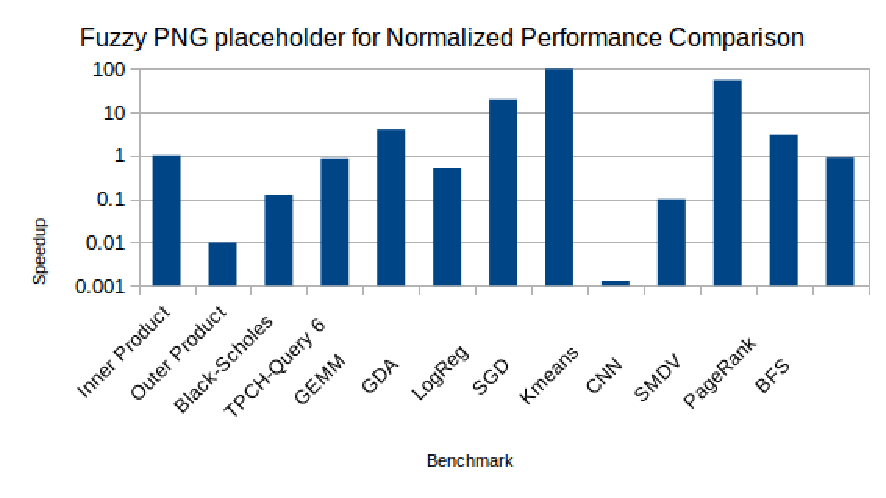
\includegraphics[width=0.45\textwidth]{figs/perf_comp.pdf}
% \caption{Comparison between run-times on Plasticine architecture versus FPGA for identical implementations of the benchmarks specified in Table~\ref{t-apps}}
% \label{fig:perf_comp}
% \end{figure}

% \begin{figure}[ht]
% \centering
% 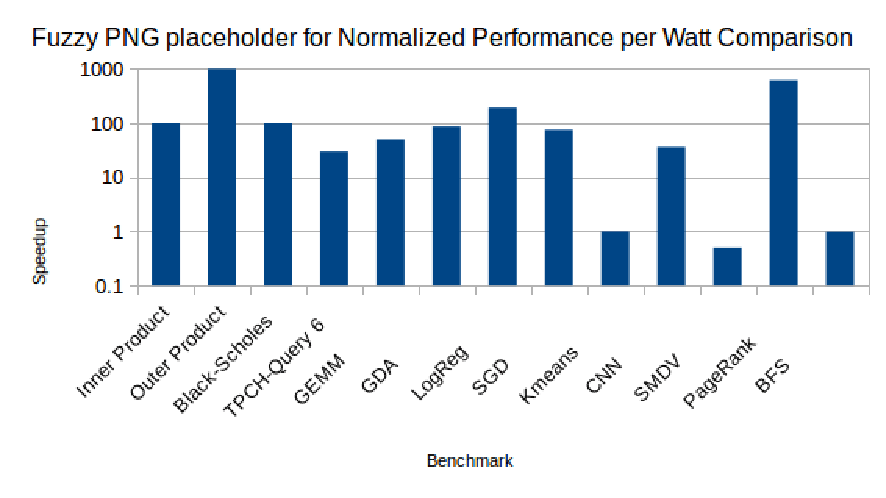
\includegraphics[width=0.45\textwidth]{figs/perf_per_watt_comp.pdf}
% \caption{Comparison between run-times on Plasticine architecture versus FPGA normalized by the power consumed by the chip for identicial implementations of the benchmarks specified in Table~\ref{t-apps}}
% \label{fig:perf_comp}
% \end{figure}


